\chapter{Bài Toán Đóng Thùng 2D - Bin Packing 2D}
\label{chap:binPacking}
%============================================================================
\section{Phát biểu bài toán}
Trong thực tế cuộc sống chúng ta rât hay gặp phải vấn đề cần giải quyết: liệu có thể xếp tất cả những vật này vào cái túi này, cái hộp này hay cái thùng kia không, lựa chọn cái nào phù hợp để vừa chứa đủ những thứ này? Các yêu cầu này nằm trong lớp bài toán đóng thùng \cite{hopper2000twodimensional}.

Để mô hình hóa tốt hơn tôi sẽ xét bài toán này trong không gian 2 chiều, khi đó các vật phẩm chỉ còn lại kích thước rộng ($w_i$) và cao $(h_i)$, và thùng có kích thước $ W \times H $. Như vậy chúng ta có bài toán đóng thùng 2 chiều (Bin Packing 2D) với phát biểu như sau:\\
Cho trước một cái thùng với kích thước $W \times H$ và $N$ vật phẩm $\{X_1,\dots,X_n\}$, các vật phẩm $X_i$ có kích thước tương ứng là $w_i \times h_i$ ($1 \leq i \leq N$). Ta cần đặt các vật phẩm (có thể xoay theo chiều ngang hoặc dọc) này vào các vị trí trong thùng sao cho các vật không chồng lấn lên nhau, không vượt khỏi biên của thùng đã cho. Câu hỏi đặt ra là liệu có một phương án sắp xếp nào đó thỏa mãn yêu cầu trên không và nếu có hãy đưa ra phương án sắp xếp đó.

%============================================================================
\section{Mô hình toán học}

\subsection*{Mô hình cơ bản}

Cho trước một cái thùng với kích thước $(W \times H)$ và $N$ vật với kích thước tương ứng được cho bởi: $(w_1, h_1),\dots,(w_n, h_n)$.\\
\textbf{Với các biến:}
\begin{align*}
	X_i &\in \{0,\dots,W-1\} \quad &1 \leq i \leq N \\
	Y_i &\in \{0,\dots,H-1\} \quad &1 \leq i \leq N \\
	R_i &\in \{0,1\} \quad &1 \leq i \leq N
\end{align*}
Các kích thước và tọa độ vật phẩm như hình ~\ref{fig:itemPositions} trong đó:
\begin{description}
	\item[$X_i$] là tọa độ theo phương ngang đặt vật thứ $i$ trong thùng.
	\item[$Y_i$] là tọa độ theo phương dọc đặt vật thứ $i$ trong thùng.
	\item[$R_i$] xác định vật phẩm được xoay hoặc không.
\end{description}

\begin{figure}[H]
	\centering
	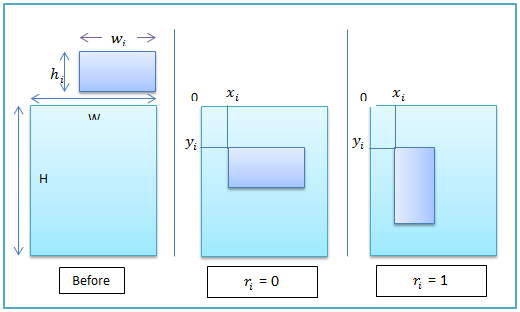
\includegraphics[scale=1]{figures/items-pos.png}
	\caption{Kích thước và tọa độ các vật phẩm\label{fig:itemPositions}}
\end{figure}

\textbf{Thỏa mãn các ràng buộc:}
\begin{align}
	C_1 &: 
	\begin{cases}
		X_i + w_i \leq W &\text{nếu } R_i = 0 \\
		X_i + h_i \leq W &\text{nếu } R_i = 1
	\end{cases}
	\\
	C_2 &: 
	\begin{cases}
		Y_i + h_i \leq H &\text{nếu } R_i = 0 \\
		Y_i + w_i \leq H &\text{nếu } R_i = 1
	\end{cases}
	\\
	C_3 &: 
	\begin{cases}
		X_i + w_i \leq X_j || X_j + w_j \leq X_i || Y_i + h_i \leq Y_j || Y_j + h_j \leq Y_i &\text{nếu }R_i = 0, R_j = 0 \\ 
		X_i + w_i \leq X_j || X_j + h_j \leq X_i || Y_i + h_i \leq Y_j || Y_j + w_j \leq Y_i &\text{nếu }R_i = 0, R_j = 1 \\ 
		X_i + h_i \leq X_j || X_j + w_j \leq X_i || Y_i + w_i \leq Y_j || Y_j + h_j \leq Y_i &\text{nếu }R_i = 1, R_j = 0 \\ 
		X_i + h_i \leq X_j || X_j + h_j \leq X_i || Y_i + w_i \leq Y_j || Y_j + w_j \leq Y_i &\text{nếu }R_i = 1, R_j = 1
	\end{cases}
\end{align}
Với:
\begin{description}
	\item[$C_1$] là ràng buộc các vật phẩm không được vượt quá biên rộng của thùng.
	\item[$C_2$] là ràng buộc các vật phẩm không được vượt quá biên cao của thùng.
	\item[$C_3$] là ràng buộc mọi vật phẩm không chồng lấn lên nhau.
\end{description}

\subsection*{Mô hình mở rộng}
Ở mô hình trước chúng ta có ba mảng chứa các biến là $X$, $Y$ và $R$, để thực hiện tìm kiếm trong mô hình tốt hơn chúng tôi đề xuất thực hiện việc gắn các biến tọa độ $x$ và $y$ với nhau thông qua một biến $pos$. Biến $pos$ này sẽ bao gồm thông tin của hai biến $x$ và $y$ như sau:
\begin{align}
	pos = y \times W + x
\end{align}
với 
\begin{itemize}
	\item[$pos$] là biến chứa thông tin tọa độ của vật trong thùng.
	\item[$x$] là biến tọa độ theo phương ngang trong thùng như ở mô hình trước.
	\item[$y$] là biến tọa độ theo phương dọc trong thùng như mô hình trước.
	\item[$W$] là chiều rộng của thùng.
\end{itemize}
Từ tọa độ $pos$ chúng ta có thể tính toán được tọa độ của các vật như sau:
\begin{align}
	\begin{cases}
		x = pos _{mode W}\\
		y = pos / W
	\end{cases}
\end{align}
%============================================================================
\section{Ứng dụng}
Bài toán đóng thùng có ứng dụng rộng rãi trong đóng gói, vận chuyển và bố trí linh kiện.
\begin{itemize}
	\item Các hãng vận chuyển thường phải xếp các vật phẩm vào các container, kích thước container là cố định nên yêu cầu cần phải xếp sao cho tiết kiệm diện tích nhất số lượng các vật phẩm cần vận chuyển.
	\item Các công ty chuyển phát nhanh cần đóng gói các gói hàng trước khi đưa lên máy bay, kích thước cho phép trên máy bay là giới hạn nên yêu cầu cần phải sắp xếp một cách tiết kiệm nhất.
	\item Phân chia các khu vực bố trí linh kiện điện tử cũng rất quan trọng bên cạnh việc nghiên cứu làm giảm kích thước linh kiện khi các thiết bị ngày nay yêu cầu nhỏ gọn mà vẫn đảm bảo hiệu năng cao, an toàn cho người sử dụng.
	\item $\dots$
\end{itemize}
